%%%%%%%%%%%%%%%%%%%%%%%%%%%%%%%%%%%%%%%%%%%%%%%%%%%%%%%%%%%%%%%%%%%%%%%%%%%
%
% Plantilla para un artículo en LaTeX en español.
%
%%%%%%%%%%%%%%%%%%%%%%%%%%%%%%%%%%%%%%%%%%%%%%%%%%%%%%%%%%%%%%%%%%%%%%%%%%%

% Qué tipo de documento estamos por comenzar:
\documentclass[a4paper]{article}
% Esto es para que el LaTeX sepa que el texto está en español:
\usepackage[spanish]{babel}
\selectlanguage{spanish}
% Esto es para poder escribir acentos directamente:
\usepackage[utf8]{inputenc}
\usepackage[T1]{fontenc}


%Qué tipo de documento estamos por comenzar:
\documentclass[a4paper]{article}
% Esto es para que el LaTeX sepa que el texto está en español:
\usepackage[spanish]{babel}
\selectlanguage{spanish}
% Esto es para poder escribir acentos directamente:
\usepackage[utf8]{inputenc}
\usepackage[T1]{fontenc}


%Qué tipo de documento estamos por comenzar:
\documentclass[a4paper]{article}
% Esto es para que el LaTeX sepa que el texto está en español:
\usepackage[spanish]{babel}
\selectlanguage{spanish}
% Esto es para poder escribir acentos directamente:
\usepackage[utf8]{inputenc}
\usepackage[T1]{fontenc}


%Qué tipo de documento estamos por comenzar:
\documentclass[a4paper]{article}
% Esto es para que el LaTeX sepa que el texto está en español:
\usepackage[spanish]{babel}
\selectlanguage{spanish}
% Esto es para poder escribir acentos directamente:
\usepackage[utf8]{inputenc}
\usepackage[T1]{fontenc}


\input{main.pdf}
%% Asigna un tamaño a la hoja y los márgenes
\usepackage[a4paper,top=3cm,bottom=2cm,left=3cm,right=3cm,marginparwidth=1.75cm]{geometry}

%% Paquetes de la AMS
\usepackage{amsmath, amsthm, amsfonts}
%% Para añadir archivos con extensión pdf, jpg, png or tif
\usepackage{graphicx}
\usepackage[colorinlistoftodos]{todonotes}
\usepackage[colorlinks=true, allcolors=blue]{hyperref}

%% Primero escribimos el título
\title{Un algoritmo de dos fases para reconocer las actividades humanas en el contexto de la Industria 4.0 y los procesos impulsados por el hombre}
\author{Borja Bordel$^1$, Ramón Alcarria$^1$, Diego Sánchez-de-Rivera$^1$\\
  \small $^1$Universidad Politécnica de Madrid, Madrid, España\\
  \small bbordel@dit.upm.es, ramon.alcarria@upm.es, diegosanchez@dit.upm.es\\
  \date{}
}

%% Después del "preámbulo", podemos empezar el documento

\begin{document}
%% Hay que decirle que incluya el título en el documento
\maketitle

%% Aquí podemos añadir un resumen del trabajo 
\begin{abstract}
\centering
Abstract.Los futuros sistemas industriales, una revolución conocida como Industria 4.0, están concebidos para integrar a las personas en el mundo cibernético como prosumidores (proveedores de servicios y consumidores). En este contexto, los procesos impulsados por el hombre aparecen como una realidad esencial y se necesitan instrumentos para crear circuitos de información de retroalimentación entre el subsistema social (personas) y el subsistema cibernético (componentes tecnológicos). Aunque se han propuesto muchos instrumentos diferentes, en la actualidad las técnicas de reconocimiento de patrones son las más prometedoras. Sin embargo, estas soluciones presentan algunos problemas importantes pendientes. Por ejemplo, dependen del hardware seleccionado para adquirir información de los usuarios; o presentan un límite en la precisión del proceso de reconocimiento. Para hacer frente a esta situación, en este trabajo se propone un algoritmo de dos fases para integrar a las personas en los sistemas de la Industria 4.0 y los procesos impulsados por el hombre. El algoritmo define acciones complejas como composiciones de movimientos simples. Las acciones complejas se reconocen utilizando modelos de Markov ocultos, y los movimientos simples se reconocen utilizando Dynamic Time Warping. De esta manera, sólo los movimientos dependen de los dispositivos de hardware empleados para capturar información, y la precisión del reconocimiento de acciones complejas se incrementa considerablemente. También se realiza una validación experimental real para evaluar y comparar el rendimiento de la solución propuesta.

Palabras Clave: Industria 4.0; reconocimiento de patrones; Warping Dinámico del Tiempo; Inteligencia Artificial; Modelos ocultos de Markov
\end{abstract}

%% Iniciamos "secciones" que servirán como subtítulos

\section{Introducci\'on}

Industria 4.0 [1] se refiere al uso de sistemas ciberfísicos (uniones de procesos físicos y cibernéticos) [2] como principal componente tecnológico de las futuras soluciones digitales, masculino (pero no sólo) en escenarios industriales. Típicamente, la digitalización ha provocado, al final, la sustitución de los mecanismos de trabajo tradicionales por nuevos instrumentos digitales. Por ejemplo, los trabajadores de las líneas de montaje fueron sustituidos por robots durante la tercera revolución industrial.
Sin embargo, algunas aplicaciones industriales no pueden basarse en soluciones tecnológicas, ya que el trabajo humano sigue siendo esencial [3]. Los productos hechos a mano son un ejemplo de aplicaciones en las que la presencia de obras humanas es esencial. En cualquier caso, estos sectores industriales deben integrarse también en la cuarta revolución industrial. De la unión de los Sistemas Cibernéticos Físicos (CPS) y los seres humanos actuando como proveedores de servicios (obras activas), surgen CPS humanizados [4]En estos nuevos sistemas se permiten procesos impulsados por el hombre [5], es decir, procesos que son conocidos, ejecutados y gestionados por personas (aunque pueden ser vigilados por mecanismos digitales).
Para crear una verdadera integración entre las personas y la tecnología, y trasladar la ejecución de los procesos del subsistema social (humanos) al mundo cibernético (componentes de hardware y software), se necesitan técnicas de extracción de información. En los últimos años se ha informado de muchas soluciones y enfoques diferentes, pero hoy en día las técnicas de reconocimiento de patrones son las más prometedoras.
El uso de Inteligencia Artificial, modelos estadísticos y otros instrumentos similares han permitido un desarrollo real e increíble de soluciones de reconocimiento de patrones, pero aún quedan algunos desafíos pendientes.
En primer lugar, las técnicas de reconocimiento de patrones dependen del dispositivo hardware subyacente para la captura de información. La estructura y el proceso de aprendizaje cambian si (por ejemplo) en lugar de los acelerómetros consideramos sensores infrarrojos. Esto es muy problemático ya que las tecnologías de hardware evolucionan mucho más rápido que las soluciones de software.
Y, segundo, hay un límite a la precisión en el proceso de reconocimiento. De hecho, a medida que las acciones humanas se vuelven más complicadas, se requieren más variables y modelos más complejos para reconocerlas. Este enfoque genera grandes problemas de optimización cuyo error residual es mayor a medida que aumenta el número de variables, lo que provoca una disminución de la tasa de reconocimiento de éxito [6]. En conclusión, las matemáticas (no el software, por lo tanto, no depende de la implementación) obligan a una cierta precisión en el proceso de reconocimiento de patrones dadas las acciones a estudiar. Para evitar esta situación, se debe considerar un menor número de variables, pero también se reduce la complejidad de las acciones que se pueden analizar, lo que resulta inaceptable en escenarios industriales donde se desarrollan actividades productivas complejas.
Por lo tanto, el objetivo de este trabajo es describir un nuevo algoritmo de reconocimiento de patrones que aborde estos dos problemas básicos. El mecanismo propuesto define las acciones como una composición de simples movimientos. Los movimientos simples se reconocen mediante técnicas de Warping Dinámico del Tiempo (DTW) [7]. Este proceso depende del hardware seleccionado para la captura de información; pero las DTW son muy flexibles y actualizar el repositorio de patrones es suficiente para reconfigurar todo el algoritmo. Luego, las acciones complejas se reconocen como combinaciones de movimientos simples a través de los Modelos Ocultos de Markov (HMM) [8]. Estos modelos son totalmente independientes de las tecnologías de hardware, ya que solo consideran acciones simples. Este enfoque en dos fases también reduce la complejidad de los modelos, aumentando la precisión y la tasa de éxito en el proceso de reconocimiento.
El resto del trabajo está organizado de la siguiente manera: en la sección 2 se describe el estado de la técnica en el reconocimiento de patrones para actividades humanas; en la sección 3 se describe la solución propuesta, incluidas las dos fases definidas; en la sección 4 se presenta una validación experimental utilizando un escenario real y usuarios finales; y en la sección 5 se concluye el trabajo.

\section{Estado de la técnica en el reconocimiento de patrones}

Se han reportado muchas técnicas diferentes de reconocimiento de patrones para actividades humanas. Sin embargo, la mayoría de las propuestas comunes se clasifican en cinco
Categorías [9]: (i) Modelos Markov Ocultos; (ii) el campo aleatorio condicional Skip Chain; (iii) Patrones Emergentes; (iv) el campo aleatorio condicional; y (v) clasificadores bayesianos.
De hecho, la mayoría de los autores proponen el uso de Modelos Ocultos de Markov (HMM) para modelar las actividades humanas. HMM permite modelar acciones como cadenas de Markov [10][11]. Básicamente, los HMM generan estados ocultos a partir de datos observables. En particular, el objetivo final de esta técnica es construir la secuencia de estados ocultos que se ajuste a una determinada secuencia de datos. Para finalmente definir todo el modelo, HMM debe deducir de los datos los parámetros del modelo de forma fiable. La Figura 1 muestra una representación esquemática de cómo funcionan los HMM. Cuando se reconocen las actividades humanas, las acciones que componen las actividades son los estados ocultos, y las salidas de los sensores son datos en estudio. HMM, además, permite el uso de técnicas de entrenamiento considerando el conocimiento previo sobre el modelo. Este entrenamiento es a veces esencial para «inducir» todas las posibles secuencias de datos requeridas para calcular el HMM. Por último, es muy importante tener en cuenta que los HMM simples aislados pueden combinarse para crear modelos más grandes y complejos.

\begin{figure}
\centering
\includegraphics[width=0.5\textwidth]\caption{\label{fig:Figura1}Representación gráfica de un HMM.}
\end{figure}

Los HMM, sin embargo, son inútiles para modelar ciertas actividades concurrentes, por lo que otros autores han reportado una nueva técnica llamada Campo Condicional Aleatorio (CRF). Los FCI se emplean para modelar aquellas actividades que presentan acciones concurrentes o, en general, múltiples acciones interactivas [12][13]. Además, HMM requiere un gran esfuerzo en el entrenamiento para descubrir todos los posibles estados ocultos. Para resolver estos problemas, el campo aleatorio condicional (CRF) emplea probabilidades condicionales en lugar de distribuciones de probabilidad conjunta. De esta manera, las actividades cuyas acciones se desarrollan en cualquier orden pueden modelarse fácilmente. A diferencia de las cadenas en HMM, CRF emplea gráficos acíclicos, y permite la integración de estados ocultos condicionales (estados que dependen de observaciones pasadas y/o futuras).
Los CRF, por otro lado, siguen siendo inútiles para modelar ciertos comportamientos, por lo que algunas propuestas generalizan este concepto y proponen el campo aleatorio condicional de la cadena de saltar (SCCRF). El SCCRF es una técnica de reconocimiento de patrones, más general que el CRF, que permite modelar actividades que no son secuenciales de acciones en la naturaleza [14]. Esta técnica trata de capturar dependencias de largo alcance (saltar cadenas); y puede entenderse como el producto de diferentes cadenas lineales. Sin embargo, el cálculo de esteproducto es bastante pesado y complicado, por lo que esta técnica suele ser demasiado costosa para ser implementada en pequeños sistemas embebidos.
Otras propuestas emplean técnicas de descripción de mayor nivel, como Emerging Patterns (EP). Para la mayoría de los autores, EP es una técnica que describe actividades como vectores de parámetros y sus valores correspondientes (localización, objeto, etc.) [15]. Utilizando distancias entre vectores es posible calcular y reconocer acciones desarrolladas por las personas. Por último, otros autores han utilizado con éxito técnicas secundarias como los clasificadores bayesianos [16], que identifican actividades que corresponden entre las actividades humanas y las salidas más probables de los sensores mientras se realizan estas acciones, considerando que todos los sensores son independientes. Árboles de decisión [17], extensiones de HMM [18] y otras tecnologías similares también han sido estudiadas en la literatura, aunque estas propuestas son escasas.
De todas las tecnologías descritas, HMM no es la más potente. Sin embargo, encaja perfectamente con la Industria 4.0, donde las acciones son muy complejas pero muy estructuradas y ordenadas (según protocolos de la empresa, políticas de eficiencia, etc.). Además, se requiere una retroalimentación rápida (a veces incluso en tiempo real) para garantizar que los procesos impulsados por el hombre funcionen correctamente antes de que se produzca un fallo crítico global. Por lo tanto, las soluciones computacionalmente costosas no son un enfoque válido, y estamos seleccionando HMM como tecnología base principal. Para preservar su ligereza y, al mismo tiempo, poder modelar actividades complejas, introducimos un sistema de reconocimiento en dos fases que permite dividir acciones complejas en dos fases más sencillas.

\section{Un algoritmo de reconocimiento de patrones en dos fases}
% 
% 
% 
% 
% 

Con el fin de (i) hacer que el proceso de reconocimiento de patrones sea independiente de los dispositivos de hardware empleados para captar información, (ii) permitir el reconocimiento de acciones complejas, y (iii) preservar el carácter ligero de los modelos seleccionados, la solución propuesta presenta una arquitectura con tres capas diferentes (véase la figura 2).

\begin{figure}
\centering
\includegraphics[width=0.5\textwidth]\caption{\label{fig:Figura2}Arquitectura de la solución propuesta de reconocimiento de patrones.}
\end{figure}

La capa inferior incluye la plataforma de hardware. Dispositivos de monitoreo como acelerómetros, smartphones, sensores infrarrojos, etiquetas RFID, etc., se implementan para capturar información sobre el comportamiento de las personas. Las salidas de estos dispositivos crean secuencias físicas de datos cuyo formato, rango dinámico, etc., dependen totalmente de las tecnologías de hardware seleccionadas.
Estas secuencias físicas de datos se procesan en la capa intermedia utilizando técnicas DTW. Como resultado, para cada secuencia física de datos, se reconoce un simple movimiento o acción. Estas acciones simples se representan utilizando un formato de datos binario para hacer la solución lo más ligera posible. El software a este nivel debe modificarse cada vez que se actualiza la plataforma de hardware, pero las tecnologías DTW no requieren un proceso de actualización pesado, y basta con actualizar el repositorio de patrones para configurar el algoritmo a este nivel.
Los movimientos simples reconocidos, entonces, se agrupan para crear secuencias de datos lógicas. Estas secuencias alimentan un sistema de reconocimiento de patrones de alto nivel basado en modelos ocultos de Markov. En este nivel, los componentes de software requieren un intenso proceso de entrenamiento, pero la capa intermedia hace totalmente independientes la plataforma de hardware y los modelos de alto nivel. Por lo tanto, cualquier cambio en la plataforma de hardware no impone una actualización en el HMM, lo que resultaría muy costoso en términos de cálculo. Mediante el análisis de la secuencia de movimientos simples, se reconocen acciones complejas.
En la subsección siguiente se describen detalladamente las dos fases propuestas de reconocimiento de patrones.

\subsection{Reconocimiento de movimiento simple: Dynamic Time Warping}

Para reconocer gestos o movimientos simples, se selecciona una solución Dynamic Time Warping. Las tecnologías DTW cumplen los requisitos de los componentes de software de nivel medio, ya que se adaptan fácilmente a las características de la plataforma de hardware subyacente y son bastante rápidas y eficientes (por lo que los pequeños dispositivos integrados pueden implementarlas).
En nuestra solución, el comportamiento humano se monitoriza mediante una familia de sensores $\delta$, que contienen componentes  $\nu_delta$  (1).

\begin{equation}
\delta = \{s_i, i = 1, ..., N_s\}
\end{equation}
Las salidas de estos sensores se muestrean periódicamente cada T_s, segundos; obteniendo
para cada instante de tiempo, t, un vector de valores N_s (cada valor de cada sensor). Esto
el vector Y_t se denomina «muestra multidimensional». (2) 
\begin{equation}
  Y_t = \{y_t^i, i = 1, ..., N_s\}
\end{equation}

Entonces, un simple movimiento Y tendrá una duración de T_m segundos y será
descrito por la secuencia temporal de muestras multidimensionales de N_m recogidas durante este tiempo (3). Para reconocer movimientos más tarde, se crea un repositorio de patrones $\real$ que contiene las secuencias temporales correspondientes para cada una de las acciones simples $\Kappa$ que deben reconocerse. (4) 

\begin{equation}
  Y = \{Y_t, t = 1, ..., T_m\} = \{Y^i, i = 1, ..., N_m\}
\end{equation}
\begin{equation}
  \Re = \{R_i, i = 1, ..., K\}
\end{equation}

En general, las personas realizan movimientos de maneras similares pero diferentes. Así pues, las transiciones pueden ser más lentas o más rápidas, pueden añadirse o suprimirse algunas acciones elementales, etc. Por lo tanto, dada una secuencia $\Chi$ con muestras Ny, que representa un movimiento a reconocer, debe estar localizado el patrón R; E R más cerca de X; por lo tanto R; se reconoce como la acción realizada. Para ello se define una función de distancia (5). Esta distancia función se puede aplicar para calcular una matriz de costos, requerido como muestras por lo general no
tienen la misma longitud ni están alineados (6).

\begin{equation}
  d: \mathcal{F} \times \mathcal{F} \rightarrow \mathbb{R},    X^i , r_j^i \in \mathcal{F}
\end{equation}

\begin{equation}
  C \in \mathbb(R)^(N_x \times N_m)  C(n,m) = d(X^n, R_j^m)
\end{equation}

En los sensores posicionales (acelerómetros, dispositivos infrarrojos, etc.), la función de distancia se aplica directamente a las salidas de los sensores (contrariamente, por ejemplo, a los micrófonos cuyas salidas deben evaluarse en el ámbito de la potencia). Aunque se pueden emplear otras funciones de distancia (la divergencia simétrica de Kullback-Leibler o la distancia de Manhattan), para este primer trabajo estamos empleando la distancia euclidiana estándar (7)

\begin{equation}
  d(X^n, R_j^m) = \sqrt{\sum_{i=1}^{N_s}(x_i^n - r_i^(m,j))^2}
\end{equation}

Entonces, se define un camino de curvatura p = (p_1, p_2, .., p_L) como una secuencia de pares (n_L,m_L) con (n_L,m_L)  € [1, N_x]x[1, N_m] y l$/isin$[1, L], satisfaciendo tres condiciones: (i)la condición límite, por ejemplo, p_1=[1,1] y p_L=[N_x,N_m]; (ii) la
condición de monotonicidad, por ejemplo, n_1≤n_2≤...≤n_L, y m_1≤m_2≤...≤m_L, y (iii) 
la condición de tamaño del escalón, por ejemplo, p_l–p_(L-1) $/isin$ {(1,0),(0,1),(1,1)} con l$/isin$[1, L–1].
Entonces, el coste total de una trayectoria de curvatura p_i se calcula sumando todos los costes parciales o distancias (8). Con todo esto, la distancia entre dos secuencias de datos $\real$_1 y $\Kappa$ está definida como el coste (distancia) de la trayectoria de curvatura óptima p* (9).

\begin{equation}
  d_p_i(X, R_j) = \sum_{l=1}^{L}d(X^n_l, R_j^m_l)
\end{equation}

\begin{equation}
  d_DTW(X,R_j) = d_p^\ast(X, R_j) = min\{d_p_i (X,R_j), siendo p_i un camino deformado\}

\end{equation}

Finalmente, el simple movimiento reconocido a partir de la secuencia de datos X es aquel cuyo
patrón R, tiene la distancia más pequeña (es la más cercana) a X. El uso de esta definición es
tolerante a las variaciones de velocidad en la ejecución del movimiento, a la introducción de nuevos
microgestos, etc. Además, como se puede ver, cuando una tecnología de hardware diferente es
implementado, basta con actualizar el repositorio de patrones R para reconfigurar toda la solución de reconocimiento de patrones (ya que no se requiere formación).

\subsection{Reconocimiento de acción compleja: Modelos ocultos de Markov}

El mecanismo propuesto anteriormente es muy útil para reconocer acciones sencillas, pero las actividades complejas implican un gran número de variables y requieren mucho más tiempo. Por lo tanto, la DTW tiende a volverse imprecisa, y se requieren modelos probabilísticos. De todos los modelos existentes, HMM es el más adecuado para escenarios industriales y procesos impulsados por el hombre.

AQUI FALTA UN PARRAFO CON LA ECUACION

Además, se hacen dos hipótesis: i) la hipótesis de Markov (14), según la cual cualquier Estado depende únicamente del anterior; y ii) la hipótesis de la independencia (15), según la cual cualquier secuencia de observación depende únicamente del Estado actual y no de estados u observaciones anteriores.

FORMULA

Para evaluar el modelo y reconocer la actividad que realizan los usuarios, en este trabajo utilizamos un enfoque tradicional (16). Aunque los algoritmos de avance han demostrado ser más eficientes, para este trabajo inicial estamos implementando directamente la expresión de evaluación en su forma tradicional.

FORMULA

El proceso de aprendizaje también se aplicó de la manera más sencilla. Se emplearon definiciones estadísticas para matriz transitoria, matriz de observación y matriz de probabilidad inicial. En particular, se utilizó la definición de probabilidad de Laplace para estimar estas tres matrices a partir de estadísticas sobre las actividades estudiadas (17-19). El operador count(∙) indica el número de veces que ocurre un evento.

FORMULA(17)


\section{Validación experimental: aplicación y resultados}

Con el fin de evaluar el desempeño de la solución propuesta, se diseñó y llevó a cabo una validación experimental. Un escenario industrial se emuló en algunas grandes salas de la Universidad Politécnica de Madrid. El escenario representaba una empresa tradicional que fabricaba productos artesanales. En particular, se emuló a un pequeño fabricante de PCB (placas de circuito impreso).
Con el fin de captar información sobre el comportamiento de las personas, los participantes recibieron un guante cibernético, incluyendo acelerómetros y un lector RFID [19]. Los objetos alrededor de los escenarios se identificaron con una etiqueta RFID, por lo que la plataforma de hardware propuesta puede identificar la posición de la mano (gesto) y los objetos con los que las personas interactúan.
Se definió y reconoció una lista de doce actividades complejas diferentes utilizando la tecnología propuesta. La Tabla 1 describe las doce actividades definidas, incluyendo una breve descripción de ellas.

%Vamos a crear la tabla.

\begin{table}[t]
\caption{\label{tab:tabla ejemplo}Descripcion de actividades complejas.}
\begin{center}
%Número de columnas:2
\begin{tabular}{ | m{2cm} | m{5cm} | }
\hline Actividad & Descripcion \\ \hline
Dibujar los caminos del circuito & El circuito a imprimir se diseña utilizando un programa informático específico para PC. \\ \hline
Imprimir el diseño del circuito usando un plotter & Utilizando lámina de plástico y una impresora especial llamada plotter, se imprime el diseño del circuito. \\ \hline
Limpiar el laminado de cobre de las tablas & Utilizando un producto especial se eliminan todo el polvo y las partículas del laminado de la cara de cobre. \\ \hline
Copiar el diseño del circuito en placas de cooper & El diseño del circuito en la lámina de plástico se copia en el laminado de cooper utilizando una ráfaga de luz UV.\\ \hline
Sumergir las tablas en la piscina de ácido & Para eliminar todo el cobre no deseado, la placa impresa se sumerge en un baño ácido.\\ \hline
Lavar el tonel con un baño de disolvente & Después del baño ácido, el resto de la superficie de cobre se lava en un baño de disolvente.\\ \hline
Alineación de capas & Los PCB se componen de varias capas; apilados y alineados durante esta fase.\\ \hline
Inspección óptica & Usando un láser, se comprueba la alineación de la capa.\\ \hline
Unir las capas exteriores con el sustrato & Utilizando un pegamento epoxi, se unen la capa final y la capa exterior de la placa.\\ \hline
Atar la junta & La unión se produce sobre una mesa de acero pesada con abrazaderas metálicas.\\ \hline
Perforar los agujeros necesarios & Se perforan agujeros para componentes, etc., en la pizarra.\\ \hline
Chapado & En un horno, la tabla está acabada.\\ \hline

\end{tabular}
\end{center}
\end{table}


Participaron en el experimento dieciocho personas (18). Se pidió a las personas que realizaran las actividades en un número aleatorio. El orden real, así como el orden en que se reconocen las actividades, fueron almacenados por un proceso de software de supervisión. Se evaluó la tasa global de éxito de toda la solución, identificando (además) la misma tasa para cada una de las fases existentes.

Para evaluar la mejoría obtenida en comparación con soluciones similares existentes, se emplearon las mismas secuencias físicas de datos para alimentar una solución estándar de reconocimiento de patrones basada únicamente en HMM. Utilizando programas informáticos de procesamiento de datos estadísticos, se extraen algunos resultados relevantes.
La Figura 4 representa la tasa media de éxito de tres casos: la solución global, la primera fase (DTW) y la segunda fase (HMM). Además, también se incluye la tasa de éxito del enfoque tradicional basado en la HMM. Como puede verse, la tecnología propuesta es, globalmente, alrededor de un 9$\%$ mejor que las técnicas tradicionales de reconocimiento de patrones basadas exclusivamente en HMM. Además, la primera fase (basada en DTW) es aproximadamente un 20$\%$ peor que la segunda fase (HMM), lo cual es significativo ya que las técnicas de Warping Dinámico del Tiempo son más débiles por defecto.

\begin{figure}
\centering
\includegraphics[width=0.5\textwidth]\caption{\label{fig:Figura3}Tasa media de éxito de la solución propuesta.}
\end{figure}

\section{Conclusiones y Futuros Trabajos}

En este trabajo presentamos un nuevo algoritmo de reconocimiento de patrones para integrar a las personas en los sistemas de la Industria 4.0 y los procesos impulsados por el hombre. El algoritmo define actividades complejas como composiciones de movimientos simples. Las actividades complejas se reconocen utilizando modelos de Markov ocultos, y los movimientos simples se reconocen utilizando Dynamic Time Warping. Para permitir la implementación de este algoritmo en pequeños dispositivos embebidos, se seleccionan configuraciones ligeras. También se lleva a cabo una validación experimental y los resultados muestran una mejora global de la tasa de éxito en torno al 9$\%$
En los trabajos futuros se considerarán las metodologías más complejas para el procesamiento de datos, y se evaluará la comparación de las diferentes configuraciones del algoritmo propuesto. Además, la propuesta se analizará en diferentes escenarios.

\begin{abstract}
\centering
Agradecimientos. La investigación que ha dado lugar a estos resultados ha recibido financiación del Ministerio de Economía y Competitividad a través del proyecto SEMOLA (TEC2015-68 284-R) y del Ministerio de Ciencia, Innovación y Universidades a través del proyecto VACADENA (RTC-2017-6031-2).
\end{abstract}




\bibliographystyle{abbrv}
\bibliography{referencias}


\blindtext

\end{document}
%% Asigna un tamaño a la hoja y los márgenes
\usepackage[a4paper,top=3cm,bottom=2cm,left=3cm,right=3cm,marginparwidth=1.75cm]{geometry}

%% Paquetes de la AMS
\usepackage{amsmath, amsthm, amsfonts}
%% Para añadir archivos con extensión pdf, jpg, png or tif
\usepackage{graphicx}
\usepackage[colorinlistoftodos]{todonotes}
\usepackage[colorlinks=true, allcolors=blue]{hyperref}

%% Primero escribimos el título
\title{Un algoritmo de dos fases para reconocer las actividades humanas en el contexto de la Industria 4.0 y los procesos impulsados por el hombre}
\author{Borja Bordel$^1$, Ramón Alcarria$^1$, Diego Sánchez-de-Rivera$^1$\\
  \small $^1$Universidad Politécnica de Madrid, Madrid, España\\
  \small bbordel@dit.upm.es, ramon.alcarria@upm.es, diegosanchez@dit.upm.es\\
  \date{}
}

%% Después del "preámbulo", podemos empezar el documento

\begin{document}
%% Hay que decirle que incluya el título en el documento
\maketitle

%% Aquí podemos añadir un resumen del trabajo 
\begin{abstract}
\centering
Abstract.Los futuros sistemas industriales, una revolución conocida como Industria 4.0, están concebidos para integrar a las personas en el mundo cibernético como prosumidores (proveedores de servicios y consumidores). En este contexto, los procesos impulsados por el hombre aparecen como una realidad esencial y se necesitan instrumentos para crear circuitos de información de retroalimentación entre el subsistema social (personas) y el subsistema cibernético (componentes tecnológicos). Aunque se han propuesto muchos instrumentos diferentes, en la actualidad las técnicas de reconocimiento de patrones son las más prometedoras. Sin embargo, estas soluciones presentan algunos problemas importantes pendientes. Por ejemplo, dependen del hardware seleccionado para adquirir información de los usuarios; o presentan un límite en la precisión del proceso de reconocimiento. Para hacer frente a esta situación, en este trabajo se propone un algoritmo de dos fases para integrar a las personas en los sistemas de la Industria 4.0 y los procesos impulsados por el hombre. El algoritmo define acciones complejas como composiciones de movimientos simples. Las acciones complejas se reconocen utilizando modelos de Markov ocultos, y los movimientos simples se reconocen utilizando Dynamic Time Warping. De esta manera, sólo los movimientos dependen de los dispositivos de hardware empleados para capturar información, y la precisión del reconocimiento de acciones complejas se incrementa considerablemente. También se realiza una validación experimental real para evaluar y comparar el rendimiento de la solución propuesta.

Palabras Clave: Industria 4.0; reconocimiento de patrones; Warping Dinámico del Tiempo; Inteligencia Artificial; Modelos ocultos de Markov
\end{abstract}

%% Iniciamos "secciones" que servirán como subtítulos

\section{Introducci\'on}

Industria 4.0 [1] se refiere al uso de sistemas ciberfísicos (uniones de procesos físicos y cibernéticos) [2] como principal componente tecnológico de las futuras soluciones digitales, masculino (pero no sólo) en escenarios industriales. Típicamente, la digitalización ha provocado, al final, la sustitución de los mecanismos de trabajo tradicionales por nuevos instrumentos digitales. Por ejemplo, los trabajadores de las líneas de montaje fueron sustituidos por robots durante la tercera revolución industrial.
Sin embargo, algunas aplicaciones industriales no pueden basarse en soluciones tecnológicas, ya que el trabajo humano sigue siendo esencial [3]. Los productos hechos a mano son un ejemplo de aplicaciones en las que la presencia de obras humanas es esencial. En cualquier caso, estos sectores industriales deben integrarse también en la cuarta revolución industrial. De la unión de los Sistemas Cibernéticos Físicos (CPS) y los seres humanos actuando como proveedores de servicios (obras activas), surgen CPS humanizados [4]En estos nuevos sistemas se permiten procesos impulsados por el hombre [5], es decir, procesos que son conocidos, ejecutados y gestionados por personas (aunque pueden ser vigilados por mecanismos digitales).
Para crear una verdadera integración entre las personas y la tecnología, y trasladar la ejecución de los procesos del subsistema social (humanos) al mundo cibernético (componentes de hardware y software), se necesitan técnicas de extracción de información. En los últimos años se ha informado de muchas soluciones y enfoques diferentes, pero hoy en día las técnicas de reconocimiento de patrones son las más prometedoras.
El uso de Inteligencia Artificial, modelos estadísticos y otros instrumentos similares han permitido un desarrollo real e increíble de soluciones de reconocimiento de patrones, pero aún quedan algunos desafíos pendientes.
En primer lugar, las técnicas de reconocimiento de patrones dependen del dispositivo hardware subyacente para la captura de información. La estructura y el proceso de aprendizaje cambian si (por ejemplo) en lugar de los acelerómetros consideramos sensores infrarrojos. Esto es muy problemático ya que las tecnologías de hardware evolucionan mucho más rápido que las soluciones de software.
Y, segundo, hay un límite a la precisión en el proceso de reconocimiento. De hecho, a medida que las acciones humanas se vuelven más complicadas, se requieren más variables y modelos más complejos para reconocerlas. Este enfoque genera grandes problemas de optimización cuyo error residual es mayor a medida que aumenta el número de variables, lo que provoca una disminución de la tasa de reconocimiento de éxito [6]. En conclusión, las matemáticas (no el software, por lo tanto, no depende de la implementación) obligan a una cierta precisión en el proceso de reconocimiento de patrones dadas las acciones a estudiar. Para evitar esta situación, se debe considerar un menor número de variables, pero también se reduce la complejidad de las acciones que se pueden analizar, lo que resulta inaceptable en escenarios industriales donde se desarrollan actividades productivas complejas.
Por lo tanto, el objetivo de este trabajo es describir un nuevo algoritmo de reconocimiento de patrones que aborde estos dos problemas básicos. El mecanismo propuesto define las acciones como una composición de simples movimientos. Los movimientos simples se reconocen mediante técnicas de Warping Dinámico del Tiempo (DTW) [7]. Este proceso depende del hardware seleccionado para la captura de información; pero las DTW son muy flexibles y actualizar el repositorio de patrones es suficiente para reconfigurar todo el algoritmo. Luego, las acciones complejas se reconocen como combinaciones de movimientos simples a través de los Modelos Ocultos de Markov (HMM) [8]. Estos modelos son totalmente independientes de las tecnologías de hardware, ya que solo consideran acciones simples. Este enfoque en dos fases también reduce la complejidad de los modelos, aumentando la precisión y la tasa de éxito en el proceso de reconocimiento.
El resto del trabajo está organizado de la siguiente manera: en la sección 2 se describe el estado de la técnica en el reconocimiento de patrones para actividades humanas; en la sección 3 se describe la solución propuesta, incluidas las dos fases definidas; en la sección 4 se presenta una validación experimental utilizando un escenario real y usuarios finales; y en la sección 5 se concluye el trabajo.

\section{Estado de la técnica en el reconocimiento de patrones}

Se han reportado muchas técnicas diferentes de reconocimiento de patrones para actividades humanas. Sin embargo, la mayoría de las propuestas comunes se clasifican en cinco
Categorías [9]: (i) Modelos Markov Ocultos; (ii) el campo aleatorio condicional Skip Chain; (iii) Patrones Emergentes; (iv) el campo aleatorio condicional; y (v) clasificadores bayesianos.
De hecho, la mayoría de los autores proponen el uso de Modelos Ocultos de Markov (HMM) para modelar las actividades humanas. HMM permite modelar acciones como cadenas de Markov [10][11]. Básicamente, los HMM generan estados ocultos a partir de datos observables. En particular, el objetivo final de esta técnica es construir la secuencia de estados ocultos que se ajuste a una determinada secuencia de datos. Para finalmente definir todo el modelo, HMM debe deducir de los datos los parámetros del modelo de forma fiable. La Figura 1 muestra una representación esquemática de cómo funcionan los HMM. Cuando se reconocen las actividades humanas, las acciones que componen las actividades son los estados ocultos, y las salidas de los sensores son datos en estudio. HMM, además, permite el uso de técnicas de entrenamiento considerando el conocimiento previo sobre el modelo. Este entrenamiento es a veces esencial para «inducir» todas las posibles secuencias de datos requeridas para calcular el HMM. Por último, es muy importante tener en cuenta que los HMM simples aislados pueden combinarse para crear modelos más grandes y complejos.

\begin{figure}
\centering
\includegraphics[width=0.5\textwidth]\caption{\label{fig:Figura1}Representación gráfica de un HMM.}
\end{figure}

Los HMM, sin embargo, son inútiles para modelar ciertas actividades concurrentes, por lo que otros autores han reportado una nueva técnica llamada Campo Condicional Aleatorio (CRF). Los FCI se emplean para modelar aquellas actividades que presentan acciones concurrentes o, en general, múltiples acciones interactivas [12][13]. Además, HMM requiere un gran esfuerzo en el entrenamiento para descubrir todos los posibles estados ocultos. Para resolver estos problemas, el campo aleatorio condicional (CRF) emplea probabilidades condicionales en lugar de distribuciones de probabilidad conjunta. De esta manera, las actividades cuyas acciones se desarrollan en cualquier orden pueden modelarse fácilmente. A diferencia de las cadenas en HMM, CRF emplea gráficos acíclicos, y permite la integración de estados ocultos condicionales (estados que dependen de observaciones pasadas y/o futuras).
Los CRF, por otro lado, siguen siendo inútiles para modelar ciertos comportamientos, por lo que algunas propuestas generalizan este concepto y proponen el campo aleatorio condicional de la cadena de saltar (SCCRF). El SCCRF es una técnica de reconocimiento de patrones, más general que el CRF, que permite modelar actividades que no son secuenciales de acciones en la naturaleza [14]. Esta técnica trata de capturar dependencias de largo alcance (saltar cadenas); y puede entenderse como el producto de diferentes cadenas lineales. Sin embargo, el cálculo de esteproducto es bastante pesado y complicado, por lo que esta técnica suele ser demasiado costosa para ser implementada en pequeños sistemas embebidos.
Otras propuestas emplean técnicas de descripción de mayor nivel, como Emerging Patterns (EP). Para la mayoría de los autores, EP es una técnica que describe actividades como vectores de parámetros y sus valores correspondientes (localización, objeto, etc.) [15]. Utilizando distancias entre vectores es posible calcular y reconocer acciones desarrolladas por las personas. Por último, otros autores han utilizado con éxito técnicas secundarias como los clasificadores bayesianos [16], que identifican actividades que corresponden entre las actividades humanas y las salidas más probables de los sensores mientras se realizan estas acciones, considerando que todos los sensores son independientes. Árboles de decisión [17], extensiones de HMM [18] y otras tecnologías similares también han sido estudiadas en la literatura, aunque estas propuestas son escasas.
De todas las tecnologías descritas, HMM no es la más potente. Sin embargo, encaja perfectamente con la Industria 4.0, donde las acciones son muy complejas pero muy estructuradas y ordenadas (según protocolos de la empresa, políticas de eficiencia, etc.). Además, se requiere una retroalimentación rápida (a veces incluso en tiempo real) para garantizar que los procesos impulsados por el hombre funcionen correctamente antes de que se produzca un fallo crítico global. Por lo tanto, las soluciones computacionalmente costosas no son un enfoque válido, y estamos seleccionando HMM como tecnología base principal. Para preservar su ligereza y, al mismo tiempo, poder modelar actividades complejas, introducimos un sistema de reconocimiento en dos fases que permite dividir acciones complejas en dos fases más sencillas.

\section{Un algoritmo de reconocimiento de patrones en dos fases}
% 
% 
% 
% 
% 

Con el fin de (i) hacer que el proceso de reconocimiento de patrones sea independiente de los dispositivos de hardware empleados para captar información, (ii) permitir el reconocimiento de acciones complejas, y (iii) preservar el carácter ligero de los modelos seleccionados, la solución propuesta presenta una arquitectura con tres capas diferentes (véase la figura 2).

\begin{figure}
\centering
\includegraphics[width=0.5\textwidth]\caption{\label{fig:Figura2}Arquitectura de la solución propuesta de reconocimiento de patrones.}
\end{figure}

La capa inferior incluye la plataforma de hardware. Dispositivos de monitoreo como acelerómetros, smartphones, sensores infrarrojos, etiquetas RFID, etc., se implementan para capturar información sobre el comportamiento de las personas. Las salidas de estos dispositivos crean secuencias físicas de datos cuyo formato, rango dinámico, etc., dependen totalmente de las tecnologías de hardware seleccionadas.
Estas secuencias físicas de datos se procesan en la capa intermedia utilizando técnicas DTW. Como resultado, para cada secuencia física de datos, se reconoce un simple movimiento o acción. Estas acciones simples se representan utilizando un formato de datos binario para hacer la solución lo más ligera posible. El software a este nivel debe modificarse cada vez que se actualiza la plataforma de hardware, pero las tecnologías DTW no requieren un proceso de actualización pesado, y basta con actualizar el repositorio de patrones para configurar el algoritmo a este nivel.
Los movimientos simples reconocidos, entonces, se agrupan para crear secuencias de datos lógicas. Estas secuencias alimentan un sistema de reconocimiento de patrones de alto nivel basado en modelos ocultos de Markov. En este nivel, los componentes de software requieren un intenso proceso de entrenamiento, pero la capa intermedia hace totalmente independientes la plataforma de hardware y los modelos de alto nivel. Por lo tanto, cualquier cambio en la plataforma de hardware no impone una actualización en el HMM, lo que resultaría muy costoso en términos de cálculo. Mediante el análisis de la secuencia de movimientos simples, se reconocen acciones complejas.
En la subsección siguiente se describen detalladamente las dos fases propuestas de reconocimiento de patrones.

\subsection{Reconocimiento de movimiento simple: Dynamic Time Warping}

Para reconocer gestos o movimientos simples, se selecciona una solución Dynamic Time Warping. Las tecnologías DTW cumplen los requisitos de los componentes de software de nivel medio, ya que se adaptan fácilmente a las características de la plataforma de hardware subyacente y son bastante rápidas y eficientes (por lo que los pequeños dispositivos integrados pueden implementarlas).
En nuestra solución, el comportamiento humano se monitoriza mediante una familia de sensores $\delta$, que contienen componentes  $\nu_delta$  (1).

\begin{equation}
\delta = \{s_i, i = 1, ..., N_s\}
\end{equation}
Las salidas de estos sensores se muestrean periódicamente cada T_s, segundos; obteniendo
para cada instante de tiempo, t, un vector de valores N_s (cada valor de cada sensor). Esto
el vector Y_t se denomina «muestra multidimensional». (2) 
\begin{equation}
  Y_t = \{y_t^i, i = 1, ..., N_s\}
\end{equation}

Entonces, un simple movimiento Y tendrá una duración de T_m segundos y será
descrito por la secuencia temporal de muestras multidimensionales de N_m recogidas durante este tiempo (3). Para reconocer movimientos más tarde, se crea un repositorio de patrones $\real$ que contiene las secuencias temporales correspondientes para cada una de las acciones simples $\Kappa$ que deben reconocerse. (4) 

\begin{equation}
  Y = \{Y_t, t = 1, ..., T_m\} = \{Y^i, i = 1, ..., N_m\}
\end{equation}
\begin{equation}
  \Re = \{R_i, i = 1, ..., K\}
\end{equation}

En general, las personas realizan movimientos de maneras similares pero diferentes. Así pues, las transiciones pueden ser más lentas o más rápidas, pueden añadirse o suprimirse algunas acciones elementales, etc. Por lo tanto, dada una secuencia $\Chi$ con muestras Ny, que representa un movimiento a reconocer, debe estar localizado el patrón R; E R más cerca de X; por lo tanto R; se reconoce como la acción realizada. Para ello se define una función de distancia (5). Esta distancia función se puede aplicar para calcular una matriz de costos, requerido como muestras por lo general no
tienen la misma longitud ni están alineados (6).

\begin{equation}
  d: \mathcal{F} \times \mathcal{F} \rightarrow \mathbb{R},    X^i , r_j^i \in \mathcal{F}
\end{equation}

\begin{equation}
  C \in \mathbb(R)^(N_x \times N_m)  C(n,m) = d(X^n, R_j^m)
\end{equation}

En los sensores posicionales (acelerómetros, dispositivos infrarrojos, etc.), la función de distancia se aplica directamente a las salidas de los sensores (contrariamente, por ejemplo, a los micrófonos cuyas salidas deben evaluarse en el ámbito de la potencia). Aunque se pueden emplear otras funciones de distancia (la divergencia simétrica de Kullback-Leibler o la distancia de Manhattan), para este primer trabajo estamos empleando la distancia euclidiana estándar (7)

\begin{equation}
  d(X^n, R_j^m) = \sqrt{\sum_{i=1}^{N_s}(x_i^n - r_i^(m,j))^2}
\end{equation}

Entonces, se define un camino de curvatura p = (p_1, p_2, .., p_L) como una secuencia de pares (n_L,m_L) con (n_L,m_L)  € [1, N_x]x[1, N_m] y l$/isin$[1, L], satisfaciendo tres condiciones: (i)la condición límite, por ejemplo, p_1=[1,1] y p_L=[N_x,N_m]; (ii) la
condición de monotonicidad, por ejemplo, n_1≤n_2≤...≤n_L, y m_1≤m_2≤...≤m_L, y (iii) 
la condición de tamaño del escalón, por ejemplo, p_l–p_(L-1) $/isin$ {(1,0),(0,1),(1,1)} con l$/isin$[1, L–1].
Entonces, el coste total de una trayectoria de curvatura p_i se calcula sumando todos los costes parciales o distancias (8). Con todo esto, la distancia entre dos secuencias de datos $\real$_1 y $\Kappa$ está definida como el coste (distancia) de la trayectoria de curvatura óptima p* (9).

\begin{equation}
  d_p_i(X, R_j) = \sum_{l=1}^{L}d(X^n_l, R_j^m_l)
\end{equation}

\begin{equation}
  d_DTW(X,R_j) = d_p^\ast(X, R_j) = min\{d_p_i (X,R_j), siendo p_i un camino deformado\}

\end{equation}

Finalmente, el simple movimiento reconocido a partir de la secuencia de datos X es aquel cuyo
patrón R, tiene la distancia más pequeña (es la más cercana) a X. El uso de esta definición es
tolerante a las variaciones de velocidad en la ejecución del movimiento, a la introducción de nuevos
microgestos, etc. Además, como se puede ver, cuando una tecnología de hardware diferente es
implementado, basta con actualizar el repositorio de patrones R para reconfigurar toda la solución de reconocimiento de patrones (ya que no se requiere formación).

\subsection{Reconocimiento de acción compleja: Modelos ocultos de Markov}

El mecanismo propuesto anteriormente es muy útil para reconocer acciones sencillas, pero las actividades complejas implican un gran número de variables y requieren mucho más tiempo. Por lo tanto, la DTW tiende a volverse imprecisa, y se requieren modelos probabilísticos. De todos los modelos existentes, HMM es el más adecuado para escenarios industriales y procesos impulsados por el hombre.

AQUI FALTA UN PARRAFO CON LA ECUACION

Además, se hacen dos hipótesis: i) la hipótesis de Markov (14), según la cual cualquier Estado depende únicamente del anterior; y ii) la hipótesis de la independencia (15), según la cual cualquier secuencia de observación depende únicamente del Estado actual y no de estados u observaciones anteriores.

FORMULA

Para evaluar el modelo y reconocer la actividad que realizan los usuarios, en este trabajo utilizamos un enfoque tradicional (16). Aunque los algoritmos de avance han demostrado ser más eficientes, para este trabajo inicial estamos implementando directamente la expresión de evaluación en su forma tradicional.

FORMULA

El proceso de aprendizaje también se aplicó de la manera más sencilla. Se emplearon definiciones estadísticas para matriz transitoria, matriz de observación y matriz de probabilidad inicial. En particular, se utilizó la definición de probabilidad de Laplace para estimar estas tres matrices a partir de estadísticas sobre las actividades estudiadas (17-19). El operador count(∙) indica el número de veces que ocurre un evento.

FORMULA(17)


\section{Validación experimental: aplicación y resultados}

Con el fin de evaluar el desempeño de la solución propuesta, se diseñó y llevó a cabo una validación experimental. Un escenario industrial se emuló en algunas grandes salas de la Universidad Politécnica de Madrid. El escenario representaba una empresa tradicional que fabricaba productos artesanales. En particular, se emuló a un pequeño fabricante de PCB (placas de circuito impreso).
Con el fin de captar información sobre el comportamiento de las personas, los participantes recibieron un guante cibernético, incluyendo acelerómetros y un lector RFID [19]. Los objetos alrededor de los escenarios se identificaron con una etiqueta RFID, por lo que la plataforma de hardware propuesta puede identificar la posición de la mano (gesto) y los objetos con los que las personas interactúan.
Se definió y reconoció una lista de doce actividades complejas diferentes utilizando la tecnología propuesta. La Tabla 1 describe las doce actividades definidas, incluyendo una breve descripción de ellas.

%Vamos a crear la tabla.

\begin{table}[t]
\caption{\label{tab:tabla ejemplo}Descripcion de actividades complejas.}
\begin{center}
%Número de columnas:2
\begin{tabular}{ | m{2cm} | m{5cm} | }
\hline Actividad & Descripcion \\ \hline
Dibujar los caminos del circuito & El circuito a imprimir se diseña utilizando un programa informático específico para PC. \\ \hline
Imprimir el diseño del circuito usando un plotter & Utilizando lámina de plástico y una impresora especial llamada plotter, se imprime el diseño del circuito. \\ \hline
Limpiar el laminado de cobre de las tablas & Utilizando un producto especial se eliminan todo el polvo y las partículas del laminado de la cara de cobre. \\ \hline
Copiar el diseño del circuito en placas de cooper & El diseño del circuito en la lámina de plástico se copia en el laminado de cooper utilizando una ráfaga de luz UV.\\ \hline
Sumergir las tablas en la piscina de ácido & Para eliminar todo el cobre no deseado, la placa impresa se sumerge en un baño ácido.\\ \hline
Lavar el tonel con un baño de disolvente & Después del baño ácido, el resto de la superficie de cobre se lava en un baño de disolvente.\\ \hline
Alineación de capas & Los PCB se componen de varias capas; apilados y alineados durante esta fase.\\ \hline
Inspección óptica & Usando un láser, se comprueba la alineación de la capa.\\ \hline
Unir las capas exteriores con el sustrato & Utilizando un pegamento epoxi, se unen la capa final y la capa exterior de la placa.\\ \hline
Atar la junta & La unión se produce sobre una mesa de acero pesada con abrazaderas metálicas.\\ \hline
Perforar los agujeros necesarios & Se perforan agujeros para componentes, etc., en la pizarra.\\ \hline
Chapado & En un horno, la tabla está acabada.\\ \hline

\end{tabular}
\end{center}
\end{table}


Participaron en el experimento dieciocho personas (18). Se pidió a las personas que realizaran las actividades en un número aleatorio. El orden real, así como el orden en que se reconocen las actividades, fueron almacenados por un proceso de software de supervisión. Se evaluó la tasa global de éxito de toda la solución, identificando (además) la misma tasa para cada una de las fases existentes.

Para evaluar la mejoría obtenida en comparación con soluciones similares existentes, se emplearon las mismas secuencias físicas de datos para alimentar una solución estándar de reconocimiento de patrones basada únicamente en HMM. Utilizando programas informáticos de procesamiento de datos estadísticos, se extraen algunos resultados relevantes.
La Figura 4 representa la tasa media de éxito de tres casos: la solución global, la primera fase (DTW) y la segunda fase (HMM). Además, también se incluye la tasa de éxito del enfoque tradicional basado en la HMM. Como puede verse, la tecnología propuesta es, globalmente, alrededor de un 9$\%$ mejor que las técnicas tradicionales de reconocimiento de patrones basadas exclusivamente en HMM. Además, la primera fase (basada en DTW) es aproximadamente un 20$\%$ peor que la segunda fase (HMM), lo cual es significativo ya que las técnicas de Warping Dinámico del Tiempo son más débiles por defecto.

\begin{figure}
\centering
\includegraphics[width=0.5\textwidth]\caption{\label{fig:Figura3}Tasa media de éxito de la solución propuesta.}
\end{figure}

\section{Conclusiones y Futuros Trabajos}

En este trabajo presentamos un nuevo algoritmo de reconocimiento de patrones para integrar a las personas en los sistemas de la Industria 4.0 y los procesos impulsados por el hombre. El algoritmo define actividades complejas como composiciones de movimientos simples. Las actividades complejas se reconocen utilizando modelos de Markov ocultos, y los movimientos simples se reconocen utilizando Dynamic Time Warping. Para permitir la implementación de este algoritmo en pequeños dispositivos embebidos, se seleccionan configuraciones ligeras. También se lleva a cabo una validación experimental y los resultados muestran una mejora global de la tasa de éxito en torno al 9$\%$
En los trabajos futuros se considerarán las metodologías más complejas para el procesamiento de datos, y se evaluará la comparación de las diferentes configuraciones del algoritmo propuesto. Además, la propuesta se analizará en diferentes escenarios.

\begin{abstract}
\centering
Agradecimientos. La investigación que ha dado lugar a estos resultados ha recibido financiación del Ministerio de Economía y Competitividad a través del proyecto SEMOLA (TEC2015-68 284-R) y del Ministerio de Ciencia, Innovación y Universidades a través del proyecto VACADENA (RTC-2017-6031-2).
\end{abstract}




\bibliographystyle{abbrv}
\bibliography{referencias}


\blindtext

\end{document}
%% Asigna un tamaño a la hoja y los márgenes
\usepackage[a4paper,top=3cm,bottom=2cm,left=3cm,right=3cm,marginparwidth=1.75cm]{geometry}

%% Paquetes de la AMS
\usepackage{amsmath, amsthm, amsfonts}
%% Para añadir archivos con extensión pdf, jpg, png or tif
\usepackage{graphicx}
\usepackage[colorinlistoftodos]{todonotes}
\usepackage[colorlinks=true, allcolors=blue]{hyperref}

%% Primero escribimos el título
\title{Un algoritmo de dos fases para reconocer las actividades humanas en el contexto de la Industria 4.0 y los procesos impulsados por el hombre}
\author{Borja Bordel$^1$, Ramón Alcarria$^1$, Diego Sánchez-de-Rivera$^1$\\
  \small $^1$Universidad Politécnica de Madrid, Madrid, España\\
  \small bbordel@dit.upm.es, ramon.alcarria@upm.es, diegosanchez@dit.upm.es\\
  \date{}
}

%% Después del "preámbulo", podemos empezar el documento

\begin{document}
%% Hay que decirle que incluya el título en el documento
\maketitle

%% Aquí podemos añadir un resumen del trabajo 
\begin{abstract}
\centering
Abstract.Los futuros sistemas industriales, una revolución conocida como Industria 4.0, están concebidos para integrar a las personas en el mundo cibernético como prosumidores (proveedores de servicios y consumidores). En este contexto, los procesos impulsados por el hombre aparecen como una realidad esencial y se necesitan instrumentos para crear circuitos de información de retroalimentación entre el subsistema social (personas) y el subsistema cibernético (componentes tecnológicos). Aunque se han propuesto muchos instrumentos diferentes, en la actualidad las técnicas de reconocimiento de patrones son las más prometedoras. Sin embargo, estas soluciones presentan algunos problemas importantes pendientes. Por ejemplo, dependen del hardware seleccionado para adquirir información de los usuarios; o presentan un límite en la precisión del proceso de reconocimiento. Para hacer frente a esta situación, en este trabajo se propone un algoritmo de dos fases para integrar a las personas en los sistemas de la Industria 4.0 y los procesos impulsados por el hombre. El algoritmo define acciones complejas como composiciones de movimientos simples. Las acciones complejas se reconocen utilizando modelos de Markov ocultos, y los movimientos simples se reconocen utilizando Dynamic Time Warping. De esta manera, sólo los movimientos dependen de los dispositivos de hardware empleados para capturar información, y la precisión del reconocimiento de acciones complejas se incrementa considerablemente. También se realiza una validación experimental real para evaluar y comparar el rendimiento de la solución propuesta.

Palabras Clave: Industria 4.0; reconocimiento de patrones; Warping Dinámico del Tiempo; Inteligencia Artificial; Modelos ocultos de Markov
\end{abstract}

%% Iniciamos "secciones" que servirán como subtítulos

\section{Introducci\'on}

Industria 4.0 [1] se refiere al uso de sistemas ciberfísicos (uniones de procesos físicos y cibernéticos) [2] como principal componente tecnológico de las futuras soluciones digitales, masculino (pero no sólo) en escenarios industriales. Típicamente, la digitalización ha provocado, al final, la sustitución de los mecanismos de trabajo tradicionales por nuevos instrumentos digitales. Por ejemplo, los trabajadores de las líneas de montaje fueron sustituidos por robots durante la tercera revolución industrial.
Sin embargo, algunas aplicaciones industriales no pueden basarse en soluciones tecnológicas, ya que el trabajo humano sigue siendo esencial [3]. Los productos hechos a mano son un ejemplo de aplicaciones en las que la presencia de obras humanas es esencial. En cualquier caso, estos sectores industriales deben integrarse también en la cuarta revolución industrial. De la unión de los Sistemas Cibernéticos Físicos (CPS) y los seres humanos actuando como proveedores de servicios (obras activas), surgen CPS humanizados [4]En estos nuevos sistemas se permiten procesos impulsados por el hombre [5], es decir, procesos que son conocidos, ejecutados y gestionados por personas (aunque pueden ser vigilados por mecanismos digitales).
Para crear una verdadera integración entre las personas y la tecnología, y trasladar la ejecución de los procesos del subsistema social (humanos) al mundo cibernético (componentes de hardware y software), se necesitan técnicas de extracción de información. En los últimos años se ha informado de muchas soluciones y enfoques diferentes, pero hoy en día las técnicas de reconocimiento de patrones son las más prometedoras.
El uso de Inteligencia Artificial, modelos estadísticos y otros instrumentos similares han permitido un desarrollo real e increíble de soluciones de reconocimiento de patrones, pero aún quedan algunos desafíos pendientes.
En primer lugar, las técnicas de reconocimiento de patrones dependen del dispositivo hardware subyacente para la captura de información. La estructura y el proceso de aprendizaje cambian si (por ejemplo) en lugar de los acelerómetros consideramos sensores infrarrojos. Esto es muy problemático ya que las tecnologías de hardware evolucionan mucho más rápido que las soluciones de software.
Y, segundo, hay un límite a la precisión en el proceso de reconocimiento. De hecho, a medida que las acciones humanas se vuelven más complicadas, se requieren más variables y modelos más complejos para reconocerlas. Este enfoque genera grandes problemas de optimización cuyo error residual es mayor a medida que aumenta el número de variables, lo que provoca una disminución de la tasa de reconocimiento de éxito [6]. En conclusión, las matemáticas (no el software, por lo tanto, no depende de la implementación) obligan a una cierta precisión en el proceso de reconocimiento de patrones dadas las acciones a estudiar. Para evitar esta situación, se debe considerar un menor número de variables, pero también se reduce la complejidad de las acciones que se pueden analizar, lo que resulta inaceptable en escenarios industriales donde se desarrollan actividades productivas complejas.
Por lo tanto, el objetivo de este trabajo es describir un nuevo algoritmo de reconocimiento de patrones que aborde estos dos problemas básicos. El mecanismo propuesto define las acciones como una composición de simples movimientos. Los movimientos simples se reconocen mediante técnicas de Warping Dinámico del Tiempo (DTW) [7]. Este proceso depende del hardware seleccionado para la captura de información; pero las DTW son muy flexibles y actualizar el repositorio de patrones es suficiente para reconfigurar todo el algoritmo. Luego, las acciones complejas se reconocen como combinaciones de movimientos simples a través de los Modelos Ocultos de Markov (HMM) [8]. Estos modelos son totalmente independientes de las tecnologías de hardware, ya que solo consideran acciones simples. Este enfoque en dos fases también reduce la complejidad de los modelos, aumentando la precisión y la tasa de éxito en el proceso de reconocimiento.
El resto del trabajo está organizado de la siguiente manera: en la sección 2 se describe el estado de la técnica en el reconocimiento de patrones para actividades humanas; en la sección 3 se describe la solución propuesta, incluidas las dos fases definidas; en la sección 4 se presenta una validación experimental utilizando un escenario real y usuarios finales; y en la sección 5 se concluye el trabajo.

\section{Estado de la técnica en el reconocimiento de patrones}

Se han reportado muchas técnicas diferentes de reconocimiento de patrones para actividades humanas. Sin embargo, la mayoría de las propuestas comunes se clasifican en cinco
Categorías [9]: (i) Modelos Markov Ocultos; (ii) el campo aleatorio condicional Skip Chain; (iii) Patrones Emergentes; (iv) el campo aleatorio condicional; y (v) clasificadores bayesianos.
De hecho, la mayoría de los autores proponen el uso de Modelos Ocultos de Markov (HMM) para modelar las actividades humanas. HMM permite modelar acciones como cadenas de Markov [10][11]. Básicamente, los HMM generan estados ocultos a partir de datos observables. En particular, el objetivo final de esta técnica es construir la secuencia de estados ocultos que se ajuste a una determinada secuencia de datos. Para finalmente definir todo el modelo, HMM debe deducir de los datos los parámetros del modelo de forma fiable. La Figura 1 muestra una representación esquemática de cómo funcionan los HMM. Cuando se reconocen las actividades humanas, las acciones que componen las actividades son los estados ocultos, y las salidas de los sensores son datos en estudio. HMM, además, permite el uso de técnicas de entrenamiento considerando el conocimiento previo sobre el modelo. Este entrenamiento es a veces esencial para «inducir» todas las posibles secuencias de datos requeridas para calcular el HMM. Por último, es muy importante tener en cuenta que los HMM simples aislados pueden combinarse para crear modelos más grandes y complejos.

\begin{figure}
\centering
\includegraphics[width=0.5\textwidth]\caption{\label{fig:Figura1}Representación gráfica de un HMM.}
\end{figure}

Los HMM, sin embargo, son inútiles para modelar ciertas actividades concurrentes, por lo que otros autores han reportado una nueva técnica llamada Campo Condicional Aleatorio (CRF). Los FCI se emplean para modelar aquellas actividades que presentan acciones concurrentes o, en general, múltiples acciones interactivas [12][13]. Además, HMM requiere un gran esfuerzo en el entrenamiento para descubrir todos los posibles estados ocultos. Para resolver estos problemas, el campo aleatorio condicional (CRF) emplea probabilidades condicionales en lugar de distribuciones de probabilidad conjunta. De esta manera, las actividades cuyas acciones se desarrollan en cualquier orden pueden modelarse fácilmente. A diferencia de las cadenas en HMM, CRF emplea gráficos acíclicos, y permite la integración de estados ocultos condicionales (estados que dependen de observaciones pasadas y/o futuras).
Los CRF, por otro lado, siguen siendo inútiles para modelar ciertos comportamientos, por lo que algunas propuestas generalizan este concepto y proponen el campo aleatorio condicional de la cadena de saltar (SCCRF). El SCCRF es una técnica de reconocimiento de patrones, más general que el CRF, que permite modelar actividades que no son secuenciales de acciones en la naturaleza [14]. Esta técnica trata de capturar dependencias de largo alcance (saltar cadenas); y puede entenderse como el producto de diferentes cadenas lineales. Sin embargo, el cálculo de esteproducto es bastante pesado y complicado, por lo que esta técnica suele ser demasiado costosa para ser implementada en pequeños sistemas embebidos.
Otras propuestas emplean técnicas de descripción de mayor nivel, como Emerging Patterns (EP). Para la mayoría de los autores, EP es una técnica que describe actividades como vectores de parámetros y sus valores correspondientes (localización, objeto, etc.) [15]. Utilizando distancias entre vectores es posible calcular y reconocer acciones desarrolladas por las personas. Por último, otros autores han utilizado con éxito técnicas secundarias como los clasificadores bayesianos [16], que identifican actividades que corresponden entre las actividades humanas y las salidas más probables de los sensores mientras se realizan estas acciones, considerando que todos los sensores son independientes. Árboles de decisión [17], extensiones de HMM [18] y otras tecnologías similares también han sido estudiadas en la literatura, aunque estas propuestas son escasas.
De todas las tecnologías descritas, HMM no es la más potente. Sin embargo, encaja perfectamente con la Industria 4.0, donde las acciones son muy complejas pero muy estructuradas y ordenadas (según protocolos de la empresa, políticas de eficiencia, etc.). Además, se requiere una retroalimentación rápida (a veces incluso en tiempo real) para garantizar que los procesos impulsados por el hombre funcionen correctamente antes de que se produzca un fallo crítico global. Por lo tanto, las soluciones computacionalmente costosas no son un enfoque válido, y estamos seleccionando HMM como tecnología base principal. Para preservar su ligereza y, al mismo tiempo, poder modelar actividades complejas, introducimos un sistema de reconocimiento en dos fases que permite dividir acciones complejas en dos fases más sencillas.

\section{Un algoritmo de reconocimiento de patrones en dos fases}
% 
% 
% 
% 
% 

Con el fin de (i) hacer que el proceso de reconocimiento de patrones sea independiente de los dispositivos de hardware empleados para captar información, (ii) permitir el reconocimiento de acciones complejas, y (iii) preservar el carácter ligero de los modelos seleccionados, la solución propuesta presenta una arquitectura con tres capas diferentes (véase la figura 2).

\begin{figure}
\centering
\includegraphics[width=0.5\textwidth]\caption{\label{fig:Figura2}Arquitectura de la solución propuesta de reconocimiento de patrones.}
\end{figure}

La capa inferior incluye la plataforma de hardware. Dispositivos de monitoreo como acelerómetros, smartphones, sensores infrarrojos, etiquetas RFID, etc., se implementan para capturar información sobre el comportamiento de las personas. Las salidas de estos dispositivos crean secuencias físicas de datos cuyo formato, rango dinámico, etc., dependen totalmente de las tecnologías de hardware seleccionadas.
Estas secuencias físicas de datos se procesan en la capa intermedia utilizando técnicas DTW. Como resultado, para cada secuencia física de datos, se reconoce un simple movimiento o acción. Estas acciones simples se representan utilizando un formato de datos binario para hacer la solución lo más ligera posible. El software a este nivel debe modificarse cada vez que se actualiza la plataforma de hardware, pero las tecnologías DTW no requieren un proceso de actualización pesado, y basta con actualizar el repositorio de patrones para configurar el algoritmo a este nivel.
Los movimientos simples reconocidos, entonces, se agrupan para crear secuencias de datos lógicas. Estas secuencias alimentan un sistema de reconocimiento de patrones de alto nivel basado en modelos ocultos de Markov. En este nivel, los componentes de software requieren un intenso proceso de entrenamiento, pero la capa intermedia hace totalmente independientes la plataforma de hardware y los modelos de alto nivel. Por lo tanto, cualquier cambio en la plataforma de hardware no impone una actualización en el HMM, lo que resultaría muy costoso en términos de cálculo. Mediante el análisis de la secuencia de movimientos simples, se reconocen acciones complejas.
En la subsección siguiente se describen detalladamente las dos fases propuestas de reconocimiento de patrones.

\subsection{Reconocimiento de movimiento simple: Dynamic Time Warping}

Para reconocer gestos o movimientos simples, se selecciona una solución Dynamic Time Warping. Las tecnologías DTW cumplen los requisitos de los componentes de software de nivel medio, ya que se adaptan fácilmente a las características de la plataforma de hardware subyacente y son bastante rápidas y eficientes (por lo que los pequeños dispositivos integrados pueden implementarlas).
En nuestra solución, el comportamiento humano se monitoriza mediante una familia de sensores $\delta$, que contienen componentes  $\nu_delta$  (1).

\begin{equation}
\delta = \{s_i, i = 1, ..., N_s\}
\end{equation}
Las salidas de estos sensores se muestrean periódicamente cada T_s, segundos; obteniendo
para cada instante de tiempo, t, un vector de valores N_s (cada valor de cada sensor). Esto
el vector Y_t se denomina «muestra multidimensional». (2) 
\begin{equation}
  Y_t = \{y_t^i, i = 1, ..., N_s\}
\end{equation}

Entonces, un simple movimiento Y tendrá una duración de T_m segundos y será
descrito por la secuencia temporal de muestras multidimensionales de N_m recogidas durante este tiempo (3). Para reconocer movimientos más tarde, se crea un repositorio de patrones $\real$ que contiene las secuencias temporales correspondientes para cada una de las acciones simples $\Kappa$ que deben reconocerse. (4) 

\begin{equation}
  Y = \{Y_t, t = 1, ..., T_m\} = \{Y^i, i = 1, ..., N_m\}
\end{equation}
\begin{equation}
  \Re = \{R_i, i = 1, ..., K\}
\end{equation}

En general, las personas realizan movimientos de maneras similares pero diferentes. Así pues, las transiciones pueden ser más lentas o más rápidas, pueden añadirse o suprimirse algunas acciones elementales, etc. Por lo tanto, dada una secuencia $\Chi$ con muestras Ny, que representa un movimiento a reconocer, debe estar localizado el patrón R; E R más cerca de X; por lo tanto R; se reconoce como la acción realizada. Para ello se define una función de distancia (5). Esta distancia función se puede aplicar para calcular una matriz de costos, requerido como muestras por lo general no
tienen la misma longitud ni están alineados (6).

\begin{equation}
  d: \mathcal{F} \times \mathcal{F} \rightarrow \mathbb{R},    X^i , r_j^i \in \mathcal{F}
\end{equation}

\begin{equation}
  C \in \mathbb(R)^(N_x \times N_m)  C(n,m) = d(X^n, R_j^m)
\end{equation}

En los sensores posicionales (acelerómetros, dispositivos infrarrojos, etc.), la función de distancia se aplica directamente a las salidas de los sensores (contrariamente, por ejemplo, a los micrófonos cuyas salidas deben evaluarse en el ámbito de la potencia). Aunque se pueden emplear otras funciones de distancia (la divergencia simétrica de Kullback-Leibler o la distancia de Manhattan), para este primer trabajo estamos empleando la distancia euclidiana estándar (7)

\begin{equation}
  d(X^n, R_j^m) = \sqrt{\sum_{i=1}^{N_s}(x_i^n - r_i^(m,j))^2}
\end{equation}

Entonces, se define un camino de curvatura p = (p_1, p_2, .., p_L) como una secuencia de pares (n_L,m_L) con (n_L,m_L)  € [1, N_x]x[1, N_m] y l$/isin$[1, L], satisfaciendo tres condiciones: (i)la condición límite, por ejemplo, p_1=[1,1] y p_L=[N_x,N_m]; (ii) la
condición de monotonicidad, por ejemplo, n_1≤n_2≤...≤n_L, y m_1≤m_2≤...≤m_L, y (iii) 
la condición de tamaño del escalón, por ejemplo, p_l–p_(L-1) $/isin$ {(1,0),(0,1),(1,1)} con l$/isin$[1, L–1].
Entonces, el coste total de una trayectoria de curvatura p_i se calcula sumando todos los costes parciales o distancias (8). Con todo esto, la distancia entre dos secuencias de datos $\real$_1 y $\Kappa$ está definida como el coste (distancia) de la trayectoria de curvatura óptima p* (9).

\begin{equation}
  d_p_i(X, R_j) = \sum_{l=1}^{L}d(X^n_l, R_j^m_l)
\end{equation}

\begin{equation}
  d_DTW(X,R_j) = d_p^\ast(X, R_j) = min\{d_p_i (X,R_j), siendo p_i un camino deformado\}

\end{equation}

Finalmente, el simple movimiento reconocido a partir de la secuencia de datos X es aquel cuyo
patrón R, tiene la distancia más pequeña (es la más cercana) a X. El uso de esta definición es
tolerante a las variaciones de velocidad en la ejecución del movimiento, a la introducción de nuevos
microgestos, etc. Además, como se puede ver, cuando una tecnología de hardware diferente es
implementado, basta con actualizar el repositorio de patrones R para reconfigurar toda la solución de reconocimiento de patrones (ya que no se requiere formación).

\subsection{Reconocimiento de acción compleja: Modelos ocultos de Markov}

El mecanismo propuesto anteriormente es muy útil para reconocer acciones sencillas, pero las actividades complejas implican un gran número de variables y requieren mucho más tiempo. Por lo tanto, la DTW tiende a volverse imprecisa, y se requieren modelos probabilísticos. De todos los modelos existentes, HMM es el más adecuado para escenarios industriales y procesos impulsados por el hombre.

AQUI FALTA UN PARRAFO CON LA ECUACION

Además, se hacen dos hipótesis: i) la hipótesis de Markov (14), según la cual cualquier Estado depende únicamente del anterior; y ii) la hipótesis de la independencia (15), según la cual cualquier secuencia de observación depende únicamente del Estado actual y no de estados u observaciones anteriores.

FORMULA

Para evaluar el modelo y reconocer la actividad que realizan los usuarios, en este trabajo utilizamos un enfoque tradicional (16). Aunque los algoritmos de avance han demostrado ser más eficientes, para este trabajo inicial estamos implementando directamente la expresión de evaluación en su forma tradicional.

FORMULA

El proceso de aprendizaje también se aplicó de la manera más sencilla. Se emplearon definiciones estadísticas para matriz transitoria, matriz de observación y matriz de probabilidad inicial. En particular, se utilizó la definición de probabilidad de Laplace para estimar estas tres matrices a partir de estadísticas sobre las actividades estudiadas (17-19). El operador count(∙) indica el número de veces que ocurre un evento.

FORMULA(17)


\section{Validación experimental: aplicación y resultados}

Con el fin de evaluar el desempeño de la solución propuesta, se diseñó y llevó a cabo una validación experimental. Un escenario industrial se emuló en algunas grandes salas de la Universidad Politécnica de Madrid. El escenario representaba una empresa tradicional que fabricaba productos artesanales. En particular, se emuló a un pequeño fabricante de PCB (placas de circuito impreso).
Con el fin de captar información sobre el comportamiento de las personas, los participantes recibieron un guante cibernético, incluyendo acelerómetros y un lector RFID [19]. Los objetos alrededor de los escenarios se identificaron con una etiqueta RFID, por lo que la plataforma de hardware propuesta puede identificar la posición de la mano (gesto) y los objetos con los que las personas interactúan.
Se definió y reconoció una lista de doce actividades complejas diferentes utilizando la tecnología propuesta. La Tabla 1 describe las doce actividades definidas, incluyendo una breve descripción de ellas.

%Vamos a crear la tabla.

\begin{table}[t]
\caption{\label{tab:tabla ejemplo}Descripcion de actividades complejas.}
\begin{center}
%Número de columnas:2
\begin{tabular}{ | m{2cm} | m{5cm} | }
\hline Actividad & Descripcion \\ \hline
Dibujar los caminos del circuito & El circuito a imprimir se diseña utilizando un programa informático específico para PC. \\ \hline
Imprimir el diseño del circuito usando un plotter & Utilizando lámina de plástico y una impresora especial llamada plotter, se imprime el diseño del circuito. \\ \hline
Limpiar el laminado de cobre de las tablas & Utilizando un producto especial se eliminan todo el polvo y las partículas del laminado de la cara de cobre. \\ \hline
Copiar el diseño del circuito en placas de cooper & El diseño del circuito en la lámina de plástico se copia en el laminado de cooper utilizando una ráfaga de luz UV.\\ \hline
Sumergir las tablas en la piscina de ácido & Para eliminar todo el cobre no deseado, la placa impresa se sumerge en un baño ácido.\\ \hline
Lavar el tonel con un baño de disolvente & Después del baño ácido, el resto de la superficie de cobre se lava en un baño de disolvente.\\ \hline
Alineación de capas & Los PCB se componen de varias capas; apilados y alineados durante esta fase.\\ \hline
Inspección óptica & Usando un láser, se comprueba la alineación de la capa.\\ \hline
Unir las capas exteriores con el sustrato & Utilizando un pegamento epoxi, se unen la capa final y la capa exterior de la placa.\\ \hline
Atar la junta & La unión se produce sobre una mesa de acero pesada con abrazaderas metálicas.\\ \hline
Perforar los agujeros necesarios & Se perforan agujeros para componentes, etc., en la pizarra.\\ \hline
Chapado & En un horno, la tabla está acabada.\\ \hline

\end{tabular}
\end{center}
\end{table}


Participaron en el experimento dieciocho personas (18). Se pidió a las personas que realizaran las actividades en un número aleatorio. El orden real, así como el orden en que se reconocen las actividades, fueron almacenados por un proceso de software de supervisión. Se evaluó la tasa global de éxito de toda la solución, identificando (además) la misma tasa para cada una de las fases existentes.

Para evaluar la mejoría obtenida en comparación con soluciones similares existentes, se emplearon las mismas secuencias físicas de datos para alimentar una solución estándar de reconocimiento de patrones basada únicamente en HMM. Utilizando programas informáticos de procesamiento de datos estadísticos, se extraen algunos resultados relevantes.
La Figura 4 representa la tasa media de éxito de tres casos: la solución global, la primera fase (DTW) y la segunda fase (HMM). Además, también se incluye la tasa de éxito del enfoque tradicional basado en la HMM. Como puede verse, la tecnología propuesta es, globalmente, alrededor de un 9$\%$ mejor que las técnicas tradicionales de reconocimiento de patrones basadas exclusivamente en HMM. Además, la primera fase (basada en DTW) es aproximadamente un 20$\%$ peor que la segunda fase (HMM), lo cual es significativo ya que las técnicas de Warping Dinámico del Tiempo son más débiles por defecto.

\begin{figure}
\centering
\includegraphics[width=0.5\textwidth]\caption{\label{fig:Figura3}Tasa media de éxito de la solución propuesta.}
\end{figure}

\section{Conclusiones y Futuros Trabajos}

En este trabajo presentamos un nuevo algoritmo de reconocimiento de patrones para integrar a las personas en los sistemas de la Industria 4.0 y los procesos impulsados por el hombre. El algoritmo define actividades complejas como composiciones de movimientos simples. Las actividades complejas se reconocen utilizando modelos de Markov ocultos, y los movimientos simples se reconocen utilizando Dynamic Time Warping. Para permitir la implementación de este algoritmo en pequeños dispositivos embebidos, se seleccionan configuraciones ligeras. También se lleva a cabo una validación experimental y los resultados muestran una mejora global de la tasa de éxito en torno al 9$\%$
En los trabajos futuros se considerarán las metodologías más complejas para el procesamiento de datos, y se evaluará la comparación de las diferentes configuraciones del algoritmo propuesto. Además, la propuesta se analizará en diferentes escenarios.

\begin{abstract}
\centering
Agradecimientos. La investigación que ha dado lugar a estos resultados ha recibido financiación del Ministerio de Economía y Competitividad a través del proyecto SEMOLA (TEC2015-68 284-R) y del Ministerio de Ciencia, Innovación y Universidades a través del proyecto VACADENA (RTC-2017-6031-2).
\end{abstract}




\bibliographystyle{abbrv}
\bibliography{referencias}


\blindtext

\end{document}
%% Asigna un tamaño a la hoja y los márgenes
\usepackage[a4paper,top=3cm,bottom=2cm,left=3cm,right=3cm,marginparwidth=1.75cm]{geometry}

%% Paquetes de la AMS
\usepackage{amsmath, amsthm, amsfonts}
%% Para añadir archivos con extensión pdf, jpg, png or tif
\usepackage{graphicx}
\usepackage[colorinlistoftodos]{todonotes}
\usepackage[colorlinks=true, allcolors=blue]{hyperref}

%% Primero escribimos el título
\title{Un algoritmo de dos fases para reconocer las actividades humanas en el contexto de la Industria 4. 0 y los procesos impulsados por el hombre}
\author{Borja Bordel$^1$, Ramón Alcarria$^1$, Diego Sánchez-de-Rivera$^1$\\
  \small $^1$Universidad Politécnica de Madrid, Madrid, España\\
  \small bbordel@dit.upm.es, ramon.alcarria@upm.es, diegosanchez@dit.upm.es\\
  \date{}
}

%% Después del "preámbulo", podemos empezar el documento

\begin{document}
%% Hay que decirle que incluya el título en el documento
\maketitle

%% Aquí podemos añadir un resumen del trabajo 
\begin{abstract}
\centering
Abstract.Los futuros sistemas industriales, una revolución conocida como Industria 4.0, están concebidos para integrar a las personas en el mundo cibernético como prosumidores (proveedores de servicios y consumidores). En este contexto, los procesos impulsados por el hombre aparecen como una realidad esencial y se necesitan instrumentos para crear circuitos de información de retroalimentación entre el subsistema social (personas) y el subsistema cibernético (componentes tecnológicos). Aunque se han propuesto muchos instrumentos diferentes, en la actualidad las técnicas de reconocimiento de patrones son las más prometedoras. Sin embargo, estas soluciones presentan algunos problemas importantes pendientes. Por ejemplo, dependen del hardware seleccionado para adquirir información de los usuarios; o presentan un límite en la precisión del proceso de reconocimiento. Para hacer frente a esta situación, en este trabajo se propone un algoritmo de dos fases para integrar a las personas en los sistemas de la Industria 4.0 y los procesos impulsados por el hombre. El algoritmo define acciones complejas como composiciones de movimientos simples. Las acciones complejas se reconocen utilizando modelos de Markov ocultos, y los movimientos simples se reconocen utilizando Dynamic Time Warping. De esta manera, sólo los movimientos dependen de los dispositivos de hardware empleados para capturar información, y la precisión del reconocimiento de acciones complejas se incrementa considerablemente. También se realiza una validación experimental real para evaluar y comparar el rendimiento de la solución propuesta.

Palabras Clave: Industria 4.0; reconocimiento de patrones; Warping Dinámico del Tiempo; Inteligencia Artificial; Modelos ocultos de Markov
\end{abstract}

%% Iniciamos "secciones" que servirán como subtítulos
%% Nota que hay otra manera de añadir acentos
\section{Introducci\'on}

Industria 4.0 [1] se refiere al uso de sistemas ciberfísicos (uniones de procesos físicos y cibernéticos) [2] como principal componente tecnológico de las futuras soluciones digitales, masculino (pero no sólo) en escenarios industriales. Típicamente, la digitalización ha provocado, al final, la sustitución de los mecanismos de trabajo tradicionales por nuevos instrumentos digitales. Por ejemplo, los trabajadores de las líneas de montaje fueron sustituidos por robots durante la tercera revolución industrial.
Sin embargo, algunas aplicaciones industriales no pueden basarse en soluciones tecnológicas, ya que el trabajo humano sigue siendo esencial [3]. Los productos hechos a mano son un ejemplo de aplicaciones en las que la presencia de obras humanas es esencial. En cualquier caso, estos sectores industriales deben integrarse también en la cuarta revolución industrial. De la unión de los Sistemas Cibernéticos Físicos (CPS) y los seres humanos actuando como proveedores de servicios (obras activas), surgen CPS humanizados [4]En estos nuevos sistemas se permiten procesos impulsados por el hombre [5], es decir, procesos que son conocidos, ejecutados y gestionados por personas (aunque pueden ser vigilados por mecanismos digitales).
Para crear una verdadera integración entre las personas y la tecnología, y trasladar la ejecución de los procesos del subsistema social (humanos) al mundo cibernético (componentes de hardware y software), se necesitan técnicas de extracción de información. En los últimos años se ha informado de muchas soluciones y enfoques diferentes, pero hoy en día las técnicas de reconocimiento de patrones son las más prometedoras.
El uso de Inteligencia Artificial, modelos estadísticos y otros instrumentos similares han permitido un desarrollo real e increíble de soluciones de reconocimiento de patrones, pero aún quedan algunos desafíos pendientes.
En primer lugar, las técnicas de reconocimiento de patrones dependen del dispositivo hardware subyacente para la captura de información. La estructura y el proceso de aprendizaje cambian si (por ejemplo) en lugar de los acelerómetros consideramos sensores infrarrojos. Esto es muy problemático ya que las tecnologías de hardware evolucionan mucho más rápido que las soluciones de software.
Y, segundo, hay un límite a la precisión en el proceso de reconocimiento. De hecho, a medida que las acciones humanas se vuelven más complicadas, se requieren más variables y modelos más complejos para reconocerlas. Este enfoque genera grandes problemas de optimización cuyo error residual es mayor a medida que aumenta el número de variables, lo que provoca una disminución de la tasa de reconocimiento de éxito [6]. En conclusión, las matemáticas (no el software, por lo tanto, no depende de la implementación) obligan a una cierta precisión en el proceso de reconocimiento de patrones dadas las acciones a estudiar. Para evitar esta situación, se debe considerar un menor número de variables, pero también se reduce la complejidad de las acciones que se pueden analizar, lo que resulta inaceptable en escenarios industriales donde se desarrollan actividades productivas complejas.
Por lo tanto, el objetivo de este trabajo es describir un nuevo algoritmo de reconocimiento de patrones que aborde estos dos problemas básicos. El mecanismo propuesto define las acciones como una composición de simples movimientos. Los movimientos simples se reconocen mediante técnicas de Warping Dinámico del Tiempo (DTW) [7]. Este proceso depende del hardware seleccionado para la captura de información; pero las DTW son muy flexibles y actualizar el repositorio de patrones es suficiente para reconfigurar todo el algoritmo. Luego, las acciones complejas se reconocen como combinaciones de movimientos simples a través de los Modelos Ocultos de Markov (HMM) [8]. Estos modelos son totalmente independientes de las tecnologías de hardware, ya que solo consideran acciones simples. Este enfoque en dos fases también reduce la complejidad de los modelos, aumentando la precisión y la tasa de éxito en el proceso de reconocimiento.
El resto del trabajo está organizado de la siguiente manera: en la sección 2 se describe el estado de la técnica en el reconocimiento de patrones para actividades humanas; en la sección 3 se describe la solución propuesta, incluidas las dos fases definidas; en la sección 4 se presenta una validación experimental utilizando un escenario real y usuarios finales; y en la sección 5 se concluye el trabajo.

\section{Estado de la técnica en el reconocimiento de patrones}

Se han reportado muchas técnicas diferentes de reconocimiento de patrones para actividades humanas. Sin embargo, la mayoría de las propuestas comunes se clasifican en cinco
Categorías [9]: (i) Modelos Markov Ocultos; (ii) el campo aleatorio condicional Skip Chain; (iii) Patrones Emergentes; (iv) el campo aleatorio condicional; y (v) clasificadores bayesianos.
De hecho, la mayoría de los autores proponen el uso de Modelos Ocultos de Markov (HMM) para modelar las actividades humanas. HMM permite modelar acciones como cadenas de Markov [10][11]. Básicamente, los HMM generan estados ocultos a partir de datos observables. En particular, el objetivo final de esta técnica es construir la secuencia de estados ocultos que se ajuste a una determinada secuencia de datos. Para finalmente definir todo el modelo, HMM debe deducir de los datos los parámetros del modelo de forma fiable. La Figura 1 muestra una representación esquemática de cómo funcionan los HMM. Cuando se reconocen las actividades humanas, las acciones que componen las actividades son los estados ocultos, y las salidas de los sensores son datos en estudio. HMM, además, permite el uso de técnicas de entrenamiento considerando el conocimiento previo sobre el modelo. Este entrenamiento es a veces esencial para «inducir» todas las posibles secuencias de datos requeridas para calcular el HMM. Por último, es muy importante tener en cuenta que los HMM simples aislados pueden combinarse para crear modelos más grandes y complejos.

\begin{figure}
\centering
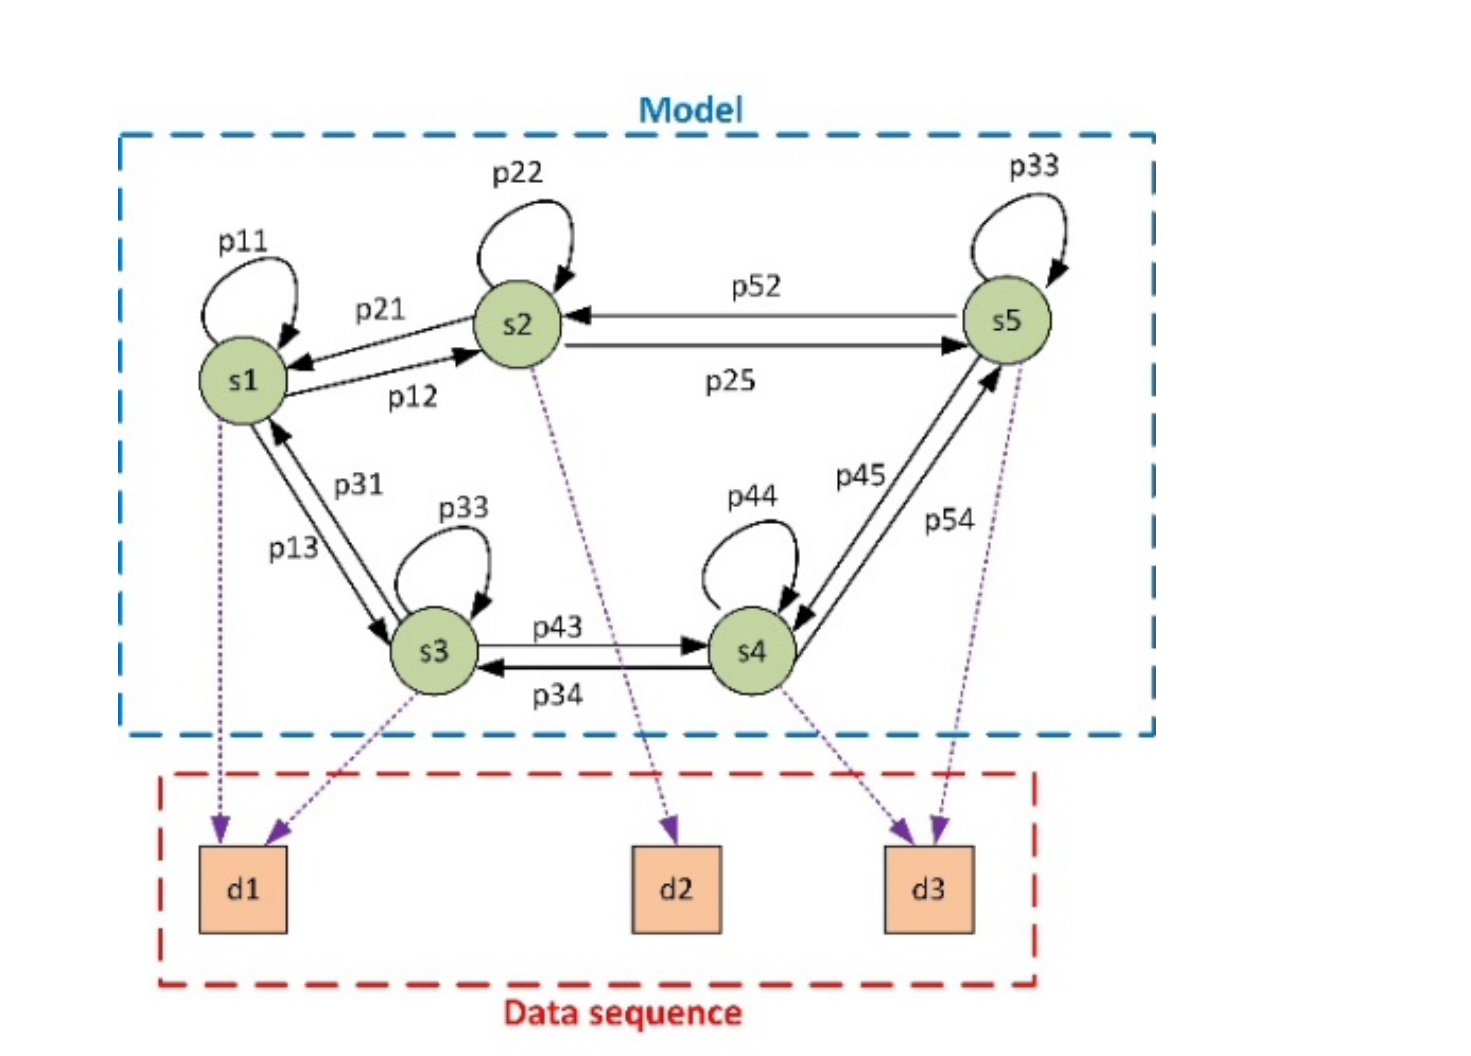
\includegraphics[width=0.5\textwidth]{Figura1.jpg}Representación gráfica de un HMM.}
\end{figure}


\subsection{¿Cómo añadir comentarios?}
% * <stephmigoni@gmail.com> 2018-02-08T19:23:33.559Z:
% 
% Esto es un comentario de prueba
% 
% 

Puedes añadir comentarios en el ícono + del menú de arriba.

Para responder a un comentario, simplemente da click en Reply en Rich Text.

También pueden añadirse comentarios en el margen del pdf compilado con el comando todo \todo{¡Comment en el margen!}, como se muestra en el ejemplo de la derecha. También puedes añadirlos dentro del texto:

\todo[inline, color=green!40]{Este es un comentario dentro del texto.}

\subsection{¿Cómo añadir tablas en mi \TeX?}

Usa los comandos table y tabular para iniciar una tabla simple --- mira la tabla~\ref{tab:tabla ejemplo}, como ejemplo. 

\begin{table}
\centering
\begin{tabular}{l c r} 
%nùmero de columnas: 3
l para left & c para centro & r para derecha \\ \hline
Ejemplo & Centrado & Alineado a la\\
Izquierda & 13 & Derecha
\end{tabular}
\caption{\label{tab:tabla ejemplo}Una simple tabla.}
\end{table}

\subsection{¿Cómo escribir (expresiones) Matemáticas?}

\LaTeX{} es buenísimo para escribir ecuaciones. Para escribir variables o ecuaciones dentro del texto lo podemos poner entre signos de pesos y luego podemos seguir escribiendo, esto funciona si queremos escribir un símbolo como $\nabla$, $\pi$, $\beta$, $\Omega$, $\aleph$, etc.
\begin{equation}
\sum_{n=0}^\infty \frac{x^n}{n!}=e^x
\end{equation}
\begin{equation}
\int_{0}^{1}dx=1
\end{equation}
\begin{equation}
e^{i\pi}+1=0
\end{equation}
Si queremos citar al gran Maxwell, lo podemos hacer como en la ecuación \ref{eq:Maxwell}:
\begin{equation}
\nabla\times\mathbf{E}+\frac{\partial\mathbf{B}}{\partial t}=0\label{eq:Maxwell}
\end{equation}

A continuación se añade un ejemplo de un desarrollo:
Con este preámbulo llevamos a cabo la siguiente transformación de los operadores $\hat{a}_{\ell}$

\begin{equation}
\hat{b}_{m}^{\dagger}=\sum_{\ell}U_{m}^{\ell}\hat{a}_{\ell}^{\dagger}
\end{equation}

donde $U_{m}^{\ell}$ es un elemento de la matriz unitaria $\mathbf{U}$.

Calculamos ahora su hermitiano conjugado
\begin{align}
\hat{b}_{m} & =\left(\sum_{\ell}U_{m}^{\ell}\hat{a}_{\ell}^{\dagger}\right)^{\dagger}\label{eq:bm}\\
 & =\sum_{\ell}\left(U_{m}^{\ell}\hat{a}_{\ell}^{\dagger}\right)^{\dagger}\nonumber \\
 & =\sum_{\ell}\left(U_{m}^{\ell}\right)^{*}\hat{a}_{\ell}\nonumber \\
 & =\sum_{\ell}\left(U^{-1}\right)_{\ell}^{m}\hat{a}_{\ell},\label{eq:bSubM}
\end{align}

Ahora, para añadir una matriz:

$$
\begin{matrix} 
a & b \\
c & d 
\end{matrix}
\quad
\begin{pmatrix} 
a & b \\
c & d 
\end{pmatrix}
\quad
\begin{bmatrix} 
a & b \\
c & d 
\end{bmatrix}
\quad
\begin{vmatrix} 
a & b \\
c & d 
\end{vmatrix}
\quad
\begin{Vmatrix} 
a & b \\
c & d 
\end{Vmatrix}
$$
%% Por ejemplo, el triple producto escalar:
\begin{equation}
\vec{A}\cdot(\vec{B}\times\vec{C})=\begin{vmatrix}
A_x&A_y&A_z\\
B_x&B_y&B_z\\
C_x&C_y&C_z\\
\end{vmatrix}
\end{equation}

\subsection{¿Cómo añadir listas?}

Puedes añadir listas con numeración automática \dots

\begin{enumerate}
\item Como esta,
\item y como esta.
\end{enumerate}
\dots o con puntitos \dots
\begin{itemize}
\item Como este,
\item y como este.
\end{itemize}

\subsection{¿Cómo añado una lista de Citas y Referencias?}

Puedes subir un archivo \verb|.bib| que contenga todas tus referencias en estilo BibTeX (puedes buscar la bibliografía de un libro en google añadiendo 'bibtex' al final), creado con JabRef. Luego podrás hacer citas así: \cite{Griffiths:1492149}.

Puedes encontrar un \href{https://www.overleaf.com/help/97-how-to-include-a-bibliography-using-bibtex}{video tutorial aquí} para aprender más acerca de BibTeX.

Espero que esta charla haya sido de tu ayuda. Puedes acceder a Overleaf en el siguiente link: \url{https://www.overleaf.com/}!

\bibliographystyle{abbrv}
\bibliography{sample}

\end{document}